\documentclass{article}
\usepackage{spconf,amsmath,amssymb,graphicx,booktabs,array}
\graphicspath{{figures_icassp/}{figures/}{../outputs/shared_error_stress/}}
% Automatically generated from outputs/icassp_primary/summary.csv.
\newcommand{\PixelFisherRange}{0.277--0.520}
\newcommand{\CaseSpearmanRange}{0.890--0.966}
\newcommand{\NAURCRange}{0.024--0.092}
\newcommand{\RRRFiftyRange}{19.3--52.1\%}

% Automatically generated from outputs/shared_error_stress/summary.csv.
\newcommand{\StressMaeIncrease}{14.9\%}
\newcommand{\StressTargetIncrease}{28.6\%}
\newcommand{\StressSharedChange}{0.0\%}
\newcommand{\StressCommitteeMaeIncrease}{11.8\%}


\title{TARGET-TO-COMMITTEE DISAGREEMENT FOR GROUND-TRUTH-FREE\\
RELIABILITY RANKING OF MRI SLICE INTERPOLATION}
\name{Anonymous Authors}
\address{Anonymous affiliation}

\begin{document}
\ninept
\maketitle

\begin{abstract}
Cohort-average reconstruction metrics cannot identify which individual MRI interpolations require review, while the true missing slices are unavailable during use. We formulate this deployment gap as ground-truth-free reliability ranking. For target interpolator $m$, we exclude $m$ from a heterogeneous committee and compute the median absolute target-to-member difference at every generated voxel; foreground aggregation produces an examination score. Ground truth is isolated from scoring and used only for retrospective evaluation. Across 161 T2-weighted examinations from IXI, fastMRI-brain, and an eight-fold out-of-fold NingXia cohort, covering ten fixed dataset--target evaluations, the score yields foreground pixel correlation \PixelFisherRange, examination-level Spearman correlation \CaseSpearmanRange, and normalized AURC \NAURCRange. We further enumerate score, normalization, mask, and committee variants and test the shared-error boundary. The method supports selective review but is not a calibrated error probability or a guarantee of clinical correctness.
\end{abstract}

\begin{keywords}
MRI interpolation, reliability ranking, selective review, model disagreement, quality control
\end{keywords}

\section{Introduction}

Through-plane interpolation converts sparsely sampled MRI volumes into denser stacks used for multiplanar visualization, registration, and volumetric analysis. Recent methods explicitly model inter-slice context, while transformer restorers provide strong image priors \cite{song2024i3net,liang2021swinir,chen2022hat}. Their evaluation is dominated by cohort-level PSNR, SSIM, and MAE. These metrics answer whether an interpolator performs well on average; they do not identify an unreliable examination after the missing slice has become unobservable.

This distinction is operationally important. A plausible-looking output may contain high reconstruction error, and a model with favorable average fidelity may fail on unusual anatomy, motion, field of view, or contrast. During deployment, direct error is unavailable. Model-internal uncertainty methods instead use Monte Carlo dropout, independently trained ensembles, heteroscedastic objectives, or learned error prediction \cite{gal2016dropout,kendall2017uncertainties,lakshminarayanan2017deepensembles,hu2021predict}. MRI-specific work has used probabilistic reconstruction, active acquisition, and deep ensembles \cite{edupuganti2021uqmri,zhang2019active,kuestner2024ensembles}. Training-free posterior inference still solves an inverse problem for each input \cite{zhang2024trainingfree}. These approaches are valuable when model internals, repeated inference, training data, or measurements are available.

Our setting is different: deterministic outputs from several existing interpolators coexist, but their internals may not. Their cross-model inconsistency is observable without the missing target. We ask whether that inconsistency can rank the error of one specified target interpolator. This differs from generic committee variance, which is a property of the set, and from no-reference MRI quality assessment, which generally predicts perceptual quality or acquisition artifacts \cite{stepien2022nriqa}. It also differs from treating heterogeneous algorithms as posterior samples.

We make three contributions. First, we formalize target-specific, ground-truth-free reliability ranking for MRI slice interpolation and define a target-to-committee score that excludes the target by identity. Second, we connect pixel error localization, examination ranking, and risk--coverage selective review in one evaluation protocol \cite{elyaniv2010selective,ding2020aurc}. Third, we evaluate when the protocol works and fails through score, intensity, mask, committee size/composition, diversity, cost, and shared-error analyses over three T2 brain cohorts. Claims are restricted to error association, ranking, selective review, and retrospective quality control.

\section{Related Work}

\subsection{Interpolation and reconstruction}
I$^3$Net combines inter- and intra-slice information for medical slice synthesis \cite{song2024i3net}. SwinIR and HAT are restoration transformers adapted here to the same through-plane interpolation task \cite{liang2021swinir,chen2022hat}. We study the stored outputs of these models and a local anatomy-consistency interpolator; improving the reconstruction architecture is outside the paper's scope. Linear and cubic interpolation provide deterministic analytical references, not putative state-of-the-art competitors.

\subsection{Uncertainty and error prediction}
Monte Carlo dropout and deep ensembles quantify variation under stochastic parameterizations or repeated training \cite{gal2016dropout,lakshminarayanan2017deepensembles}. Heteroscedastic formulations distinguish data and model uncertainty \cite{kendall2017uncertainties}; MRI work has evaluated these ideas under domain shift \cite{kuestner2024ensembles}. Hu \emph{et al.} instead learn a separate predictor of MRI reconstruction error and emphasize systematic error that variance estimators may miss \cite{hu2021predict}. Our protocol neither learns error labels nor estimates a posterior. It uses diversity among heterogeneous point reconstructions as a target-specific ranking signal.

\subsection{No-reference quality and selective prediction}
No-reference image-quality methods infer quality without a pristine image, often from learned natural-image or MRI artifact statistics \cite{stepien2022nriqa}. MRI QC has also learned heteroscedastic, task-specific quality signals from simulated k-space artifacts \cite{shaw2020heteroscedastic}. Such methods require training labels or assumptions about distortions and need not isolate the error of a named interpolator. Selective prediction formalizes the trade-off between retained coverage and risk \cite{elyaniv2010selective,geifman2019selectivenet}. AURC is preferable to a single failure threshold because it evaluates all referral workloads and accounts for retained error \cite{ding2020aurc}. We adopt this continuous ranking view; binary top-decile failure detection is secondary.

\section{Method}

\subsection{Deployment setting}
Let $x$ denote the observed sparse-slice context and $y$ the unobserved dense target. Interpolator $m$ produces $\hat y_m=f_m(x)$. Available output identities form $\mathcal B$. The target-specific committee is
\begin{equation}
 \mathcal C_m=\{\hat y_b:b\in\mathcal B,\ b\neq m\}.
 \label{eq:committee}
\end{equation}
All outputs must correspond to the same examination, voxel grid, affine, orientation, shape, generated-slice indices, and intensity representation. Ground truth is absent from Eq.~\eqref{eq:committee} and every scoring operation.

\begin{figure}[t]
 \centering
 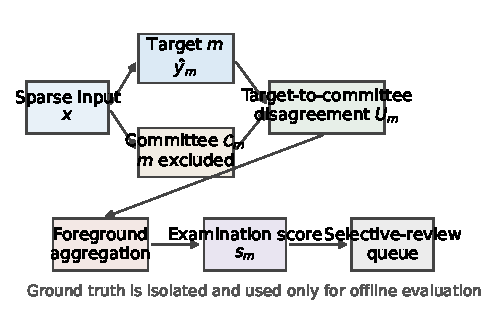
\includegraphics[width=\columnwidth]{figure_framework.pdf}
 \caption{Deployment and offline evaluation. The target is excluded from its heterogeneous committee. Ground truth is revealed only after scoring.}
 \label{fig:framework_ext}
\end{figure}

\subsection{Target-specific disagreement}
For generated voxel $i$, the default map is
\begin{equation}
 U_m(i)=\mathop{\mathrm{median}}_{b\in\mathcal C_m}
 |\hat y_m(i)-\hat y_b(i)|.
 \label{eq:disagreement_ext}
\end{equation}
We call this median target-to-committee disagreement. It is not the statistical median absolute deviation, which is centered at a sample median. Self-exclusion is essential: including $\hat y_m$ adds a structural zero and changes the estimator. The median is a pre-specified robust default, not assumed a priori to dominate the mean.

We compare target-member mean, maximum, trimmed mean, distance to the committee mean, and distance to the committee median image. Non-target-specific comparators are standard deviation over all outputs and mean/median pairwise disagreement. Analytical comparators are residuals to linear, cubic, their mean/minimum/maximum, and structural variants apply Eq.~\eqref{eq:disagreement_ext} to gradient magnitude or Laplacian responses.

\subsection{Foreground aggregation}
Only generated slices are evaluated. Let $\mathcal Z_g=\{z:z\bmod4\neq0\}$ and $\mathcal G=\{i:i_z\in\mathcal Z_g\}$ denote their voxel set. The default deployment mask is
\begin{equation}
 M_m(i)=\mathbf1\!\left[|\hat y_m(i)|>0.01\max_{j\in\mathcal G}|\hat y_m(j)|\right].
 \label{eq:mask_ext}
\end{equation}
The examination score is
\begin{equation}
 s_m=\frac{\sum_{i\in\mathcal G}M_m(i)U_m(i)}
 {\sum_{i\in\mathcal G}M_m(i)}.
 \label{eq:case_ext}
\end{equation}
The mask suppresses background but can omit tissue that the target itself suppresses. We therefore test target thresholds 0.5, 1, 2, and 5\%; committee union, intersection, and median-image masks; and a mask propagated from observed anchor slices. A 1\% ground-truth-derived mask is included only as an offline sensitivity upper bound; it is rejected by the deployment-mask API and is not a deployment method.

\subsection{Error decomposition and identifiability}
Write a reconstruction as
\begin{equation}
 \hat y_b=y+c+\epsilon_b,
 \label{eq:model_ext}
\end{equation}
where $c$ is an error common to all interpolators and $\epsilon_b$ is member specific. Then
\begin{equation}
 \hat y_m-\hat y_b=\epsilon_m-\epsilon_b.
 \label{eq:cancellation_ext}
\end{equation}
The common error cancels exactly. Thus, disagreement is sensitive when target error creates observable separation from at least part of a diverse committee. It is unidentifiable when all methods produce the same structural deletion, inherit the same bias, or are corrupted by the same preprocessing. This is an observation about Eq.~\eqref{eq:cancellation_ext}, not a theorem that disagreement recovers absolute error.

\subsection{Selective review metrics}
Offline error is $e_m(i)=|\hat y_m(i)-y(i)|$ and examination foreground MAE is $E_m$. Examinations are sorted by increasing $s_m$. At retained coverage $q$, $A_q$ contains the lowest-score fraction and $R(q)=|A_q|^{-1}\sum_{j\in A_q}E_j$. We report raw AURC, oracle AURC, random AURC, and
\begin{equation}
 \mathrm{nAURC}=\frac{\mathrm{AURC}-\mathrm{AURC}_{\rm oracle}}
 {\mathrm{AURC}_{\rm random}-\mathrm{AURC}_{\rm oracle}}.
\end{equation}
The RRR at $q$ is $[R_{\rm random}-R(q)]/R_{\rm random}$. Coverage always means retained fraction; $1-q$ is referred.

\section{Experimental Setup}

\subsection{Cohorts and interpolators}
IXI contributes 115 held-out T2 examinations and outputs from I$^3$Net, HAT, SwinIR, and ACSI \cite{ixi}. fastMRI-brain contributes 24 T2 examinations and the first three neural models \cite{zbontar2018fastmri}. NingXia is an internal cohort of 22 T2 examinations evaluated with the same three neural models through eight-fold held-out prediction; every examination is scored out of fold. Linear and cubic interpolation are computed for every profile. In total, 161 examinations form ten fixed dataset--target evaluations.

The study uses stored NIfTI outputs and does not retrain any model. Every true target is removed according to the factor-four sampling pattern and only synthesized indices are evaluated. Public or de-identified data are used; dataset-specific ethics wording will be finalized with the submission metadata.

\subsection{Alignment and intensity}
Before scoring, exact case-set equality is checked for every model and analytical output. Missing, extra, duplicate, non-finite, shape-mismatched, affine-mismatched, or orientation-mismatched files raise an error. Source NIfTI files are read only. Existing inference pipelines normalize each source volume and inversely map predictions to its original intensity range; model-specific clipping can nevertheless alter location or scale. Sensitivity experiments independently normalize each prediction by foreground p1--p99, median/IQR, or min--max statistics, using no ground truth.

\subsection{Committees, governance, and statistics}
The frozen primary specification is all available non-target members, Eq.~\eqref{eq:disagreement_ext}, raw inverse-normalized intensity, Eq.~\eqref{eq:mask_ext}, seed 20260715, and 2,000 case-bootstrap replicates. All dataset results had already been observed; variants are reported as retrospective sensitivity analyses, not used to select a different method for fastMRI-brain or NingXia.

For each target, every legal nonempty committee subset is recomputed from voxel maps. We summarize each size $k$ by mean, median, worst, best, and range over subsets. Composition labels distinguish neural, analytical, and mixed committees; output pairwise disagreement is a deployment-available diversity proxy. Real error correlation is discussed only as offline analysis. SwinIR flip-TTA remains a model-specific auxiliary comparator because equivalent TTA outputs do not exist for every target.

Pixel Pearson correlation is calculated per examination within foreground and aggregated by Fisher $z$; median/IQR and all-pixel correlation are sensitivities. Examination ranking uses Spearman $\rho$ and Kendall $\tau$. Risk--coverage includes raw, oracle, and random AURC; nAURC; RRR25/50/75; and absolute retained MAE. Paired comparisons reuse bootstrap indices. As a secondary analysis, the exact highest-MAE $\lceil0.1n\rceil$ examinations define failures for AUROC/AUPRC, giving only 12, 3, and 3 positives per target on IXI, fastMRI-brain, and NingXia. Mask variants change the MAE support and therefore receive point/interval sensitivity summaries rather than an invalid paired nAURC difference against a different endpoint.

\section{Results}

\subsection{Primary error association and ranking}
\begin{table*}[t]
 \centering
 \caption{Pre-specified all-member median disagreement. Pixel $r_z$ is the inverse Fisher-$z$ mean of per-examination foreground correlations. Lower nAURC is better. MAE$_{50}$ is an absolute retained risk and is not compared across cohort intensity scales.}
 \resizebox{\textwidth}{!}{\begin{tabular}{llrrrrrr}
\toprule
Dataset & Target & $n$ & Pixel $r_z$ & Case $\rho$ [95\% CI] & nAURC [95\% CI] & RRR$_{50}$ & MAE$_{50}$ \\
\midrule
fastMRI-brain & HAT & 24 & 0.328 & 0.916 [0.758, 0.962] & 0.067 [0.017, 0.176] & 19.7\% & 69.47 \\
fastMRI-brain & I$^3$Net & 24 & 0.291 & 0.890 [0.713, 0.966] & 0.092 [0.029, 0.194] & 19.3\% & 55.96 \\
fastMRI-brain & SwinIR & 24 & 0.363 & 0.931 [0.781, 0.978] & 0.061 [0.012, 0.150] & 20.5\% & 70.23 \\
\midrule
IXI & ACSI & 115 & 0.435 & 0.954 [0.925, 0.972] & 0.035 [0.018, 0.060] & 50.1\% & 23.51 \\
IXI & HAT & 115 & 0.512 & 0.966 [0.940, 0.980] & 0.024 [0.012, 0.042] & 49.6\% & 24.72 \\
IXI & I$^3$Net & 115 & 0.351 & 0.951 [0.922, 0.969] & 0.044 [0.024, 0.073] & 52.1\% & 18.71 \\
IXI & SwinIR & 115 & 0.520 & 0.965 [0.937, 0.980] & 0.025 [0.012, 0.044] & 49.5\% & 24.92 \\
\midrule
NingXia & HAT & 22 & 0.277 & 0.929 [0.790, 0.975] & 0.076 [0.016, 0.228] & 22.2\% & 113.54 \\
NingXia & I$^3$Net & 22 & 0.356 & 0.914 [0.769, 0.970] & 0.063 [0.016, 0.186] & 23.1\% & 124.74 \\
NingXia & SwinIR & 22 & 0.279 & 0.936 [0.807, 0.983] & 0.036 [0.007, 0.120] & 21.4\% & 115.01 \\
\bottomrule
\end{tabular}
}
 \label{tab:main_ext}
\end{table*}

Table~\ref{tab:main_ext} reports all ten profiles rather than a range over methods. Foreground spatial association is moderate (\PixelFisherRange), while examination ranking is strong (\CaseSpearmanRange). The gap is plausible: averaging disagreement over many generated voxels suppresses local noise and can rank total examination error even when the map does not precisely identify every erroneous structure. Background exclusion prevents empty voxels from carrying the localization claim.

\begin{table*}[t]
 \centering
 \caption{Secondary highest-MAE-decile failure detection. Small positive counts make these thresholded endpoints less stable than risk--coverage and examination ranking.}
 \resizebox{0.82\textwidth}{!}{\begin{tabular}{llrrr}
\toprule
Dataset & Target & Positives & AUROC [95\% CI] & AUPRC [95\% CI] \\
\midrule
fastMRI-brain & HAT & 3 & 1.000 [0.865, 1.000] & 1.000 [0.478, 1.000] \\
fastMRI-brain & I$^3$Net & 3 & 1.000 [0.810, 1.000] & 1.000 [0.477, 1.000] \\
fastMRI-brain & SwinIR & 3 & 1.000 [0.849, 1.000] & 1.000 [0.533, 1.000] \\
\midrule
IXI & ACSI & 12 & 0.991 [0.946, 1.000] & 0.949 [0.751, 1.000] \\
IXI & HAT & 12 & 0.993 [0.945, 1.000] & 0.953 [0.762, 1.000] \\
IXI & I$^3$Net & 12 & 0.983 [0.951, 0.998] & 0.863 [0.678, 0.983] \\
IXI & SwinIR & 12 & 0.992 [0.939, 1.000] & 0.951 [0.752, 1.000] \\
\midrule
NingXia & HAT & 3 & 0.982 [0.895, 1.000] & 0.917 [0.587, 1.000] \\
NingXia & I$^3$Net & 3 & 0.930 [0.789, 1.000] & 0.810 [0.420, 1.000] \\
NingXia & SwinIR & 3 & 0.982 [0.895, 1.000] & 0.917 [0.554, 1.000] \\
\bottomrule
\end{tabular}
}
 \label{tab:failure_ext}
\end{table*}

Table~\ref{tab:failure_ext} reports the thresholded view without using it as a primary claim. The three positives per target in each smaller cohort make AUROC and especially AUPRC sensitive to individual examinations; the continuous selective-review analysis below is therefore the principal deployment endpoint.

\begin{table}[t]
 \centering
 \caption{Foreground versus all-generated-voxel spatial association, averaged over fixed target profiles. The all-pixel result is secondary because background can dominate.}
 \resizebox{\columnwidth}{!}{\begin{tabular}{lrrr}
\toprule
Dataset & Foreground $r_z$ & All-pixel $r_z$ & Difference \\
\midrule
fastMRI-brain & 0.327 & 0.488 & +0.160 \\
IXI & 0.455 & 0.593 & +0.138 \\
NingXia & 0.304 & 0.474 & +0.169 \\
\bottomrule
\end{tabular}
}
 \label{tab:pixel_support_ext}
\end{table}

\subsection{Selective review}
\begin{figure*}[t]
 \centering
 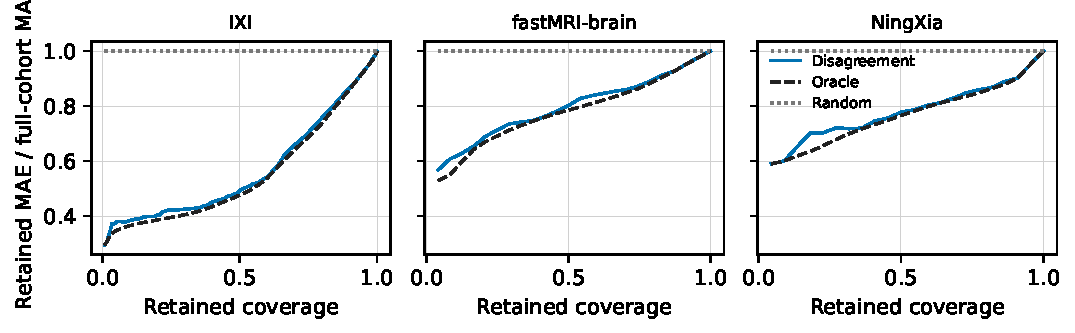
\includegraphics[width=0.96\textwidth]{figure_risk_coverage.pdf}
 \caption{Primary risk--coverage curves, normalized by full-cohort MAE and averaged over target models within each cohort. Oracle and random policies are interpretive bounds.}
 \label{fig:risk_ext}
\end{figure*}

nAURC ranges from \NAURCRange; at 50\% retained coverage the score lowers retained MAE by \RRRFiftyRange\ relative to random review. Figure~\ref{fig:risk_ext} shows that score-based referral lies between random and oracle across cohorts. The operating point is not tuned on a test cohort: 25, 50, and 75\% are all retained in the machine-readable output.

\subsection{Score, normalization, and mask sensitivity}
The complete generated tables cover all score, normalization, and mask variants. Median is not uniquely responsible for performance: mean target difference, shared standard deviation, and pairwise mean give similar average rankings, and no alternative has an exploratory paired nAURC interval excluding zero in its favor across a fixed profile. Score-rank stability is at least 0.979 in aggregate, although several variants are worse on individual profiles. Independently normalizing every output severely degrades ranking, especially on IXI, and can reverse examination order; the common source-intensity representation must therefore be preserved. Input- and committee-derived masks remain close to the default, while high target thresholds reorder fastMRI-brain cases. No variant is selected separately for any cohort.

\begin{table*}[t]
 \centering
 \begin{minipage}[t]{0.49\textwidth}
  \centering
  \caption{Normalization sensitivity relative to raw intensity. Stability is Spearman correlation between examination scores.}
  \resizebox{\linewidth}{!}{\begin{tabular}{llrrr}
\toprule
Dataset & Normalization & Mean $\Delta$nAURC & Mean stability & Minimum \\
\midrule
fastMRI-brain & minmax & +0.248 & 0.804 & 0.762 \\
fastMRI-brain & percentile\_p1\_p99 & +0.412 & 0.739 & 0.663 \\
fastMRI-brain & raw & +0.000 & 1.000 & 1.000 \\
fastMRI-brain & robust\_median\_iqr & +0.417 & 0.472 & 0.456 \\
IXI & minmax & +1.359 & -0.251 & -0.263 \\
IXI & percentile\_p1\_p99 & +1.347 & -0.198 & -0.272 \\
IXI & raw & +0.000 & 1.000 & 1.000 \\
IXI & robust\_median\_iqr & +1.212 & 0.143 & 0.097 \\
NingXia & minmax & +0.346 & 0.659 & 0.596 \\
NingXia & percentile\_p1\_p99 & +0.327 & 0.668 & 0.500 \\
NingXia & raw & +0.000 & 1.000 & 1.000 \\
NingXia & robust\_median\_iqr & +0.955 & -0.299 & -0.409 \\
\bottomrule
\end{tabular}
}
  \label{tab:norm_stability_ext}
 \end{minipage}\hfill
 \begin{minipage}[t]{0.49\textwidth}
  \centering
  \caption{Mask-induced score-ranking stability relative to the 1\% target mask. No paired error-endpoint claim is made.}
  \resizebox{\linewidth}{!}{\begin{tabular}{llrr}
\toprule
Dataset & Mask & Mean stability & Minimum \\
\midrule
fastMRI-brain & committee\_intersection & 0.983 & 0.977 \\
fastMRI-brain & committee\_median & 0.982 & 0.975 \\
fastMRI-brain & committee\_union & 0.979 & 0.973 \\
fastMRI-brain & ground\_truth\_offline & 0.985 & 0.979 \\
fastMRI-brain & input\_derived & 0.989 & 0.983 \\
fastMRI-brain & target\_0.005 & 0.881 & 0.838 \\
fastMRI-brain & target\_0.01 & 1.000 & 1.000 \\
fastMRI-brain & target\_0.02 & 0.859 & 0.812 \\
fastMRI-brain & target\_0.05 & 0.662 & 0.606 \\
IXI & committee\_intersection & 0.995 & 0.995 \\
IXI & committee\_median & 0.999 & 0.998 \\
IXI & committee\_union & 0.998 & 0.996 \\
IXI & ground\_truth\_offline & 0.994 & 0.993 \\
IXI & input\_derived & 0.996 & 0.996 \\
IXI & target\_0.005 & 0.991 & 0.990 \\
IXI & target\_0.01 & 1.000 & 1.000 \\
IXI & target\_0.02 & 0.984 & 0.983 \\
IXI & target\_0.05 & 0.979 & 0.979 \\
NingXia & committee\_intersection & 0.999 & 0.999 \\
NingXia & committee\_median & 1.000 & 0.999 \\
NingXia & committee\_union & 0.995 & 0.994 \\
NingXia & ground\_truth\_offline & 0.998 & 0.998 \\
NingXia & input\_derived & 0.998 & 0.997 \\
NingXia & target\_0.005 & 1.000 & 0.999 \\
NingXia & target\_0.01 & 1.000 & 1.000 \\
NingXia & target\_0.02 & 0.999 & 0.999 \\
NingXia & target\_0.05 & 0.999 & 0.999 \\
\bottomrule
\end{tabular}
}
  \label{tab:mask_stability_ext}
 \end{minipage}
\end{table*}

Tables~\ref{tab:norm_stability_ext} and \ref{tab:mask_stability_ext} confirm this distinction: normalization stability ranges down to negative values, whereas input/committee-mask stability is 0.973 or higher across profile means. Threshold sensitivity is concentrated on fastMRI-brain (minimum stability 0.606 at 5\%).

\IfFileExists{tables_icassp/table_tta_fastmri.tex}{%
\begin{table}[t]
 \centering
 \caption{Local fastMRI-brain SwinIR comparison under the same examination-level protocol. TTA uses four flip views and is not averaged with targets for which maps are unavailable.}
 \resizebox{\columnwidth}{!}{\begin{tabular}{lrrrrr}
\toprule
Score & Pixel $r_z$ & $\rho$ & nAURC & RRR$_{50}$ & Extra s/case \\
\midrule
Target-to-committee & 0.363 & 0.931 & 0.061 & 20.5\% & stored \\ 
Four-view TTA variance & 0.306 & 0.960 & 0.023 & 20.5\% & 1.10 \\ 
\bottomrule
\end{tabular}
}
 \label{tab:tta_ext}
\end{table}
}{ }

The stored fastMRI-brain TTA maps provide one strong single-model baseline on exactly 24 SwinIR examinations. TTA attains $\rho=0.960$ and nAURC 0.023 versus 0.931 and 0.061 for target-to-committee scoring, while its pixel association is lower (0.306 versus 0.363). The paired nAURC difference is $-0.038$ [95\% CI $-0.119$, 0.001], so the apparent gain is not conclusive at this sample size. Equivalent maps are unavailable for I$^3$Net, HAT, or ACSI. TTA also requires four forward views; target-to-committee scoring is post-hoc only when peer predictions already exist.

\subsection{Committee size, composition, and diversity}
\begin{figure}[t]
 \centering
 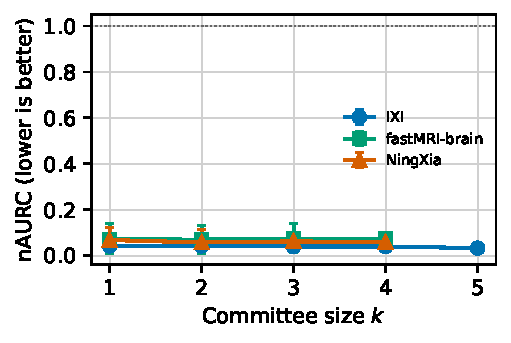
\includegraphics[width=\columnwidth]{figure_committee_size.pdf}
 \caption{Mean and subset range of nAURC by committee size. Every legal subset is recomputed at voxel level.}
 \label{fig:size_ext}
\end{figure}

\begin{table*}[t]
 \centering
 \caption{Key ablations averaged over fixed target profiles. Score columns use the full committee; composition columns use all available members of the stated type. Lower nAURC is better. Complete subset ranges remain in generated CSV files.}
 \resizebox{0.82\textwidth}{!}{\begin{tabular}{lrrrrrr}
\toprule
Dataset & Median & Mean & Shared std. & Neural-only & Analytical-only & Full \\
\midrule
fastMRI-brain & 0.073 & 0.070 & 0.074 & 0.017 & 0.118 & 0.073 \\
IXI & 0.032 & 0.043 & 0.049 & 0.033 & 0.059 & 0.032 \\
NingXia & 0.058 & 0.056 & 0.033 & 0.094 & 0.031 & 0.058 \\
\bottomrule
\end{tabular}
}
 \label{tab:key_ablation_ext}
\end{table*}

Table~\ref{tab:key_ablation_ext} exposes the cost--robustness trade-off without retrospectively selecting a member. Complete subset results report mean, median, best, worst, and range at every $k$; a favorable category mean is insufficient when an unfavorable peer performs poorly.

Figure~\ref{fig:size_ext} shows no monotone universal size law. Two neural peers are strongest on fastMRI-brain (mean nAURC 0.017) and IXI (0.029), while analytical-only is strongest on NingXia (0.031 when both analytical members are used). Adding analytical members can therefore help or hurt depending on cohort. Moreover, the output-diversity proxy has only weak association with nAURC ($\rho=-0.141$ to 0.085), so it cannot safely select a subset without labels. No single compact committee preserves full-set behavior across cohorts; the frozen all-member default is a governance choice, not an empirical optimum.

\subsection{Shared-error stress test}
\begin{figure}[t]
 \centering
 \includegraphics[width=\columnwidth]{shared_error_stress.pdf}
 \caption{Controlled additive patch corruption over 20 pre-specified IXI examinations and four targets. Bands are 95\% case-bootstrap intervals. Target-specific corruption separates the target from peers; shared corruption cancels from target-member differences.}
\label{fig:stress_ext}
\end{figure}

The stress test uses the first 20 sorted IXI test identities, all four targets, a consensus-derived foreground patch, and five fixed strengths. Target-specific corruption adds the bias only to $\hat y_m$; shared corruption adds the identical bias to every output. The default mask is frozen before corruption. This experiment does not simulate all clinical errors. It tests the algebraic boundary in Eq.~\eqref{eq:cancellation_ext}: target-specific error should raise both MAE and disagreement, whereas shared error can raise MAE while disagreement changes little.

At maximum strength, target MAE increases by \StressMaeIncrease\ in both arms. Under shared corruption, mean committee MAE also increases by \StressCommitteeMaeIncrease, yet shared-error disagreement changes by only \StressSharedChange; target-specific disagreement instead increases by \StressTargetIncrease. Thus the experiment exposes false reassurance under a controlled common-mode error rather than claiming coverage of clinical failure modes.

\subsection{Automatically selected failure examples}
\begin{figure*}[t]
 \centering
 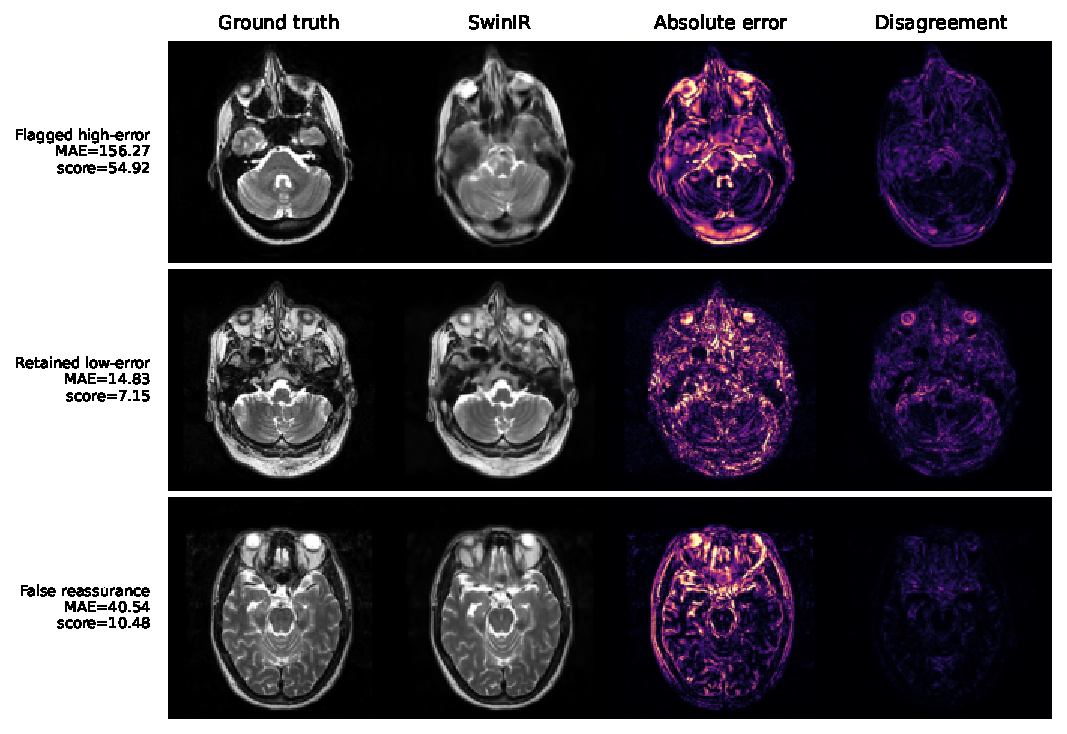
\includegraphics[width=0.65\textwidth]{figure4_committee_qualitative.pdf}
 \caption{Predefined IXI SwinIR selections from the prior asset generator: highest-error flagged examination, low-error retained examination, and highest-error false reassurance among low-score examinations. The displayed generated slice maximizes slice-wise MAE within each selected examination; error and disagreement share a row-wise scale.}
 \label{fig:failure_ext}
\end{figure*}

Figure~\ref{fig:failure_ext} separates useful referral, useful retention, and false reassurance without hand-selecting a visually attractive slice. The final row is the practical counterpart of the shared-error argument: low disagreement cannot certify that preserved consensus is correct. Conversely, high disagreement can prioritize an examination that contains unusual but accurate detail, creating unnecessary review.

\subsection{Deployment cost}
The pipeline records bytes read, scoring time for each examination and specification, output storage, and environment metadata. Scoring stored outputs is CPU post-processing and does not require model weights. This is deployment scenario A: retrospective audit when reconstructions already exist. We additionally benchmark linear and cubic interpolation on the fixed first ten examinations of each cohort, timing interpolation alone and excluding NIfTI I/O. Scenario B requires online committee generation; its cost is the sum of all selected model inference costs plus scoring. Historical model runs do not provide a complete, hardware-matched peak-GPU-memory and latency benchmark, so we do not claim that online use is free. Analytical members can run on CPU, while each neural peer requires its own reconstruction or cached output. The committee-size analysis therefore serves jointly as a ranking and cost curve.

\begin{table}[t]
 \centering
 \caption{Measured post-hoc cost. $^a$CPU interpolation only on 10 fixed examinations per cohort; NIfTI I/O excluded. Ground-truth I/O is excluded throughout.}
 \resizebox{\columnwidth}{!}{\begin{tabular}{lr}
\toprule
Measured post-hoc quantity & Value \\
\midrule
Stored-output audit / examination, mean & 1.184 s \\ 
Stored-output audit / examination, p95 & 2.872 s \\ 
NIfTI prediction load / examination, mean & 0.308 s \\ 
Score and mask kernel / examination, mean & 0.873 s \\ 
Stored deployment outputs / examination & 39.4 MiB \\ 
Observed CPU RSS peak & 0.89 GiB \\ 
Linear CPU interpolation / examination$^{a}$ & 0.046 s \\ 
Cubic CPU interpolation / examination$^{a}$ & 0.075 s \\ 
\bottomrule
\end{tabular}
}
 \label{tab:cost_ext}
\end{table}

\clearpage
\section{Discussion}

\subsection{Why examination ranking exceeds pixel localization}
Local absolute error depends on fine anatomy, registration, and intensity. Different interpolators may agree on the broad structure yet differ in the exact location of error, limiting voxel correlation. Examination aggregation averages many local comparisons and can preserve monotone between-case severity. This is why a moderate pixel result and strong case Spearman are not contradictory, but neither permits a claim of precise lesion localization.

\subsection{Target specificity versus committee spread}
Shared committee standard deviation is unchanged when the evaluation target changes; it describes the set. Equation~\eqref{eq:disagreement_ext} asks how far one named target lies from alternatives and must change with $m$. This distinction matters for model-specific quality control and for comparing interpolators on the same examination. Heterogeneous committee members are not exchangeable posterior draws, and the magnitude of $s_m$ is not a probability.

\subsection{When cross-model disagreement is useful}
The protocol is attractive when several deterministic outputs already exist, model internals are unavailable, or one audit interface must span architectures. It can complement TTA and learned error prediction: TTA measures within-model sensitivity to transformations, while cross-model disagreement probes between-interpolator behavior. If only one model can be run, TTA, posterior sampling, acquisition residuals, or a validated error predictor may be more economical.

\subsection{Limitations}
Shared structural errors are invisible by construction. Committee members may be highly correlated because they share data, losses, preprocessing, or restoration priors. Running peers online adds computation and storage. fastMRI-brain and NingXia are small, especially for top-decile failure detection. The evidence is restricted to T2 brain MRI and factor four; no broader ``across MRI settings'' claim is made. An intensity-derived foreground mask is not a clinical anatomy mask and may omit target-suppressed tissue. MAE is not diagnostic harm. There is no reader study or downstream task. High disagreement can reflect correct but unusual detail, while low disagreement can reflect common over-smoothing. Finally, the score is not probability calibrated and does not establish clinical safety.

\section{Reproducibility}
One YAML-controlled entry point validates inputs and emits per-examination scores/errors, pixel summaries, risk--coverage points, bootstrap samples, summary CSV, runtime records, environment metadata, and the result registry. Score and mask APIs have no ground-truth argument; oracle rankings reside only in evaluation code. Unit tests cover self-exclusion, size-one committees, missing examinations, score independence from ground truth, oracle/random nAURC behavior, normalization finiteness, and ordering invariance. All tables and figures in both manuscripts are generated from the same CSV outputs.

\section{Conclusion}
We presented a target-specific, ground-truth-free reliability-ranking protocol for MRI slice interpolation. Median target-to-committee disagreement can be computed from heterogeneous deterministic outputs and used to prioritize examination review. Its utility depends on member diversity, composition, masks, and intensity alignment. Shared errors remain fundamentally undetectable; the score is neither a calibrated probability nor a guarantee of clinical correctness.

\clearpage
\section*{Compliance statement}
IXI and fastMRI are public research datasets. \textbf{Author confirmation required before submission:} state NingXia access, de-identification, and ethics approval or waiver identifiers, and insert the funding declaration. No clinical decision was made from the reported scores.

\bibliographystyle{IEEEbib}
\bibliography{references}
\end{document}
